\documentclass{article}
\usepackage[ruled, linesnumbered]{algorithm2e}
\usepackage{amsmath, amsthm, amssymb, tikz, float}

\usepackage{listings}
\lstset{
  basicstyle=\ttfamily,
  columns=fullflexible
}

\usetikzlibrary{arrows,automata, positioning}

\newtheorem{thm}{Theorem}
\newtheorem{lem}[thm]{Lemma}
\newtheorem{cor}[thm]{Corollary}
\newtheorem{alg}[thm]{Algorithm}

\theoremstyle{definition}
\newtheorem{defn}[thm]{Definition}
\numberwithin{thm}{subsection}

\newcommand{\W}{\mathcal{W}}
\newcommand{\Z}{\mathbb{Z}}
\newcommand{\T}{\text{T}}



\title{Temporal Graphs Research at Pomona College\\
  \textit{Working Definitions and Vocabulary}
}
\author{Campbell, Wollman, Wu}

\begin{document}

\maketitle

\section{About}

As we continue researching temporal graphs and their related properties there is
an increased need to establish fundamental definitions. Although many papers
have established definitions of the terms and concepts contained within this
paper, there are subtle details of each of these definitions that vary from
paper to paper making it difficult to efficiently communicate exact ideas.

This document shall serve as an ongoing record of the definitions we will use
in our research. The definitions contained within should serve as the defaults
in conversations; if you intend to use an alternate definition to a concept
defined in this document, you should state and/or cite the alternate definition.
(In the future, we will look to incorporate alternate definitions in this
document as well.) It should be noted that these definitions may change as we
continue our research.

\section{Preliminary Definitions}

\begin{defn}
  A \textbf{temporal graph} or \textbf{temporal network}\footnote{We will treat
  the terms \textit{graph} and \textit{network} synonymously throughout this
  paper.} is defined as a tuple $G = (V,E,\T,\W)$ where $V$ is the set of
  vertices, and $E \subset V^2$ is the set of edges. A graph is \textbf{directed}
  if $(u,v) \in E$ is an ordered pair, and is \textbf{undirected} if unordered.

  $\T$ is a function $\T : E \to \Z^2$ with the co-domain being the start and
  end times of the vertices, in number of time units (you can always pick a
  smaller time unit so that the bounds of this interval are integral). Note that
  forall $e \in E$ with $\T(e) = (t_s, t_f)$, $t_s \leq t_f$. In a
  \textbf{static} graph, where $\T(e) = (\infty, \infty)$ for all $e \in E$,
  leave $\T$ out of the definition of the graph. $\W$ is a function

  $\W : E \to \Z$ representing the integer weight of each edge. In an
  \textbf{unweighted} graph if every edge has the same weight, then we can
  leave $\W$ out of the definition.

  All edges are to be treated as directed edges with some weight $\W$ and
  time-window $\T$ (possibly instantaneous) in which they are \textit{active}.
  Additionally, we will maintain the standard definitions of \textit{size} and
  \textit{order} defined respectively: $|E| = m$,  $|V| = n$.
\end{defn}

With this generalized definition of a temporal network, we will begin to explain
some common, specialized descriptors of these networks:

Note that there is a direct transformation between undirected temporal graphs and
directed temporal networks. Simply remove the direction of the edges, i.e. make
the ordered pairs unordered.  This is called the \textbf{underlying graph}.

\begin{defn}
  We will describe a temporal graph as \textbf{unweighted} if every edge in $E$
  has equal weight $w$.
\end{defn}

\begin{defn}
  \textbf{Edge persistence} is the amount of time for which an edge is present.
  More formally, in a graph $(V,E,\T,\W)$ the persistence of an edge $e$
  is defined, for $T(e) = (t_s,t_f)$, as $|T(e)| = t_f - t_s$.
\end{defn}

\begin{defn}
  An edge $e \in E$ is said to be \textbf{infinitely persistent} if
  $T(e) = (t_s, \infty)$.
\end{defn}

\begin{defn}
  A \textbf{instantaneous edge} or \textbf{contact edge} is any edge $e \in E$
  where $|T(e)| = 0$.
\end{defn}

\begin{defn}
  \textbf{Windowed networks} shall be defined as any temporal network where
  there is an edge $e$ with $|\T(e)| \neq 0$.
\end{defn}

\begin{defn}
  \textbf{Contact networks} shall be defined as a temporal network where
  every edge in the network is an \textit{instantaneous edge} or \textit{contact
  edge}. It is simply a special case of an interval network.
\end{defn}

\begin{defn}
  An \textbf{infinitely-edge-persisting network} shall be defined as a temporal
  network where every edge is \textbf{infinitely persistent}.
\end{defn}

\begin{defn}
  A \textbf{co-authorship network} is an undirected interval network in which
  each node represents an author, and the existence of an edge between two nodes
  represents a collaboration over the a period of time. Unless stated otherwise,
  we shall assume a \textit{collaboration} to mean two authors $a_1$ and $a_2$
  worked on (at least) one publication together in $\T(a_1,a_2)$.
\end{defn}

\begin{defn}
  A \textbf{citation network} is a directed interval network \\ $(V,E,\T,\W)$
  with infinite edge persistence. For simplicity, we can write edges as
  $u \to_{t_1} v$ or $(u,v)_{t_1}$, with $(t_1,\infty) = \T(u,v)$. In this
  network, each node represents an author, and the existence of an edge
  $u \to_{t_1} v$ means that author $v$ cited author $u$ at time $t$. This way
  the direction of the arrow represents the flow of information.
\end{defn}


Now we will move on to consider the different analysis methodologies that will
result from different temporal definitions of `shortest path'.

\begin{defn}
  A graph is a \textbf{path} if it is a simple graph whose vertices can be
  linearly ordered such that there is an edge $uv$ if and only if $u$ and $v$
  are adjacent in the ordering.
  A digraph is a \textbf{path} if it is a simple directed graph whose vertices
  can be linearly ordered such that there is an edge $u \to v$ if and only if
  $v$ immediately follows $u$ in the ordering.
\end{defn}

\begin{defn}
 A static \textbf{shortest path} between $u,v$ in a static (di)graph
 $G = (V,E,\W)$ is $P = e_1 = (u,u'), e_2, \cdots, e_n = (v',v)$,
 $P \in E$ such that for all $e_i = (v_1,v_2), e_{i+1} = (v_3,v_4) \in E$,
 $v_2 = v_3$, and for every $u,v$-path $P' = e'_1, e'_2, \cdots, e'_m$
  \[\sum_{e'_i \in P'} \W(e'_i) < \sum_{e_i \in P} \W(e_i) \]
 \end{defn}

Note that this definition does not enforce uniqueness of shortest paths.

\section{Consecutive Contemporaneity}

Here, we consider the addition of paths to include a temporal component, where
any two consecutive edges must share some contemporary period. This is a sensible
definition as two edges should not be able to form a path in a temporal network
if they did not happen at the same time. This is formally defined below.

\begin{defn}
  \label{defn:cons_temp_path}
  A \textbf{consecutive temporal path} between $u$ and $v$ at time $t$ is a $t,v_1,v_n$-path
  $P = e_1, e_2, \cdots, e_n$ such that for consecutive edges $e_i,e_{i+1} \in P$,
  $T(e_i) \cap T(e_j) \neq \emptyset$, and $t \in T(e_1)$.
\end{defn}

We will consider the consequences of this definition in the context of different
edge-behaviors, infinite persistence, and windowed persistence.

\subsection{Infinitely Persistent Edges}

The first model we will consider is the simplest of the three, where we disallow
edge-deletion. We will define the persistent coauthorship network to have this
property. [note about semantic equivalence to railway network?]

\begin{defn}
  The \textbf{persistent co-authorship network} a co-authorship network $G = (V,E)$,
  where for all $(u,v,t_1,t_2) \in E$, $t_2 = \infty$. For simplicity, we can
  denote an edge by $(u,v)_{t_1}$ or $u -_{t_1} v$. Since this network is
  undirected, $(u,v)_{t_1} = (v,u)_{t_1}$.
\end{defn}

\begin{figure}[ht] \centering
  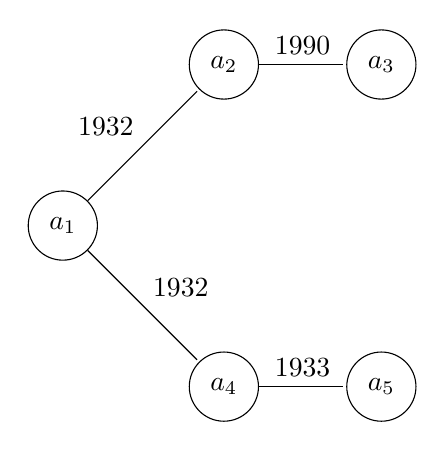
\begin{tikzpicture}[>=stealth',shorten >=1pt,auto,node distance=2cm]
    \node[state]     (a1)                            {$a_1$};
    \node[state]     (a2)     [above right=of a1]    {$a_2$};
    \node[state]     (a3)     [right of=a2]          {$a_3$};
    \node[state]     (a4)     [below right=of a1]    {$a_4$};
    \node[state]     (a5)     [right of=a4]          {$a_5$};

    \path[-]
      (a1) edge             node {1932} (a2)
           edge             node {1932} (a4)
      (a2) edge             node {1990} (a3)
      (a4) edge             node {1933} (a5);
  \end{tikzpicture}
  \caption{Example motivating the difference in shortest vs. fastest path}
  \label{fig:infinite_edge_ex}
\end{figure}

Then, we can consider what a reasonable definition of `shortest path' might be.
In this model, once an edge exists, it is always traversible, so if author
$a_1$ wrote a paper with author $a_2$ in 1932, and author $a_2$ wrote a paper with
$a_3$ in 1990, we can find a path between $a_1$ and $a_3$.  It is also feasible
that $a_1$ wrote a paper with $a_4$ in 1932 as well, and then $a_4$ and $a_5$
wrote a paper in 1933. These two paths $P_1 = a_1 -_{1932} a_2 -_{1990} a_3$, and
$P_2 = a_1 -_{1932} a_4 -_{1933} a_5$ should have some manner of differentation,
since the difference in start times of the edges is 58 in $P_1$ and only 1
in $P_1$. This can be seen in Figure \ref{fig:infinite_edge_ex}, to motivates a
difference in `fastest' vs. `shortest' path.


\begin{defn}

  \label{defn:short_fast_path}

  The \textbf{temporal shortest path} between $u$ and $v$ at time $t$ is a consecutive
  temporal $t,u,v$-path $P = e_1, \cdots, e_n$ such that that there is no other
  path $u,v$-path $P = e'_1, \cdots, e_m$ where
  \[\sum_{e'_i \in P'} \W(e'_i) < \sum_{e_i \in P} \W(e_i) \]

  The \textbf{temporal fastest path} from $v_1$ to $v_n$ at time $t$ is a consecutive
  temporal path $v_1,v_2,\cdots,v_n$, with first edge $(v_1,v_2)_{t_1}$ and last
  edge $(v_{n-1},v_n)_{t_{n-1}}$, such that there exists no other
  $u_1,u_2, \cdots, u_m$ with first edge $(u_1,u_2)_{s_1}$, last edge
  $(u_{m-1},u_m)_{s_{m-1}}$ and $s_{m-1} - s_1 < t_{n-1} - t_{1}$.
\end{defn}


\begin{cor}
  Shortest path in persistent coauthorship network is the same as the shortest
  path in the aggregated static graph.
\end{cor}

\begin{proof}[Proof. (Idea)]
  Since the edges have infinite persistence, can just wait at a vertex until
  the desired edge in the aggregated graph shows up.
\end{proof}


\subsection{Windowed edges}

Now consider that we in fact limit the persistence of the edges with an endpoint
specific to each edge (as is specified in the definition of an interval network
temporal graph). We call this graph a \textbf{windowed co-authorship network} or
simply a \textbf{co-authorship network}. If we specify a universal
edge-persistence $\Delta t$ such that for all edges $e$ in the
network, $\Delta t = |T(e)|$, then we call this co-authorship network
\textbf{$\Delta t$-windowed}.

The definitions for temporal paths will be the same as for infinitely persistent
edges, \ref{defn:cons_temp_path}. As well as those for fastest and shortest path
will be the same as in definition \ref{defn:short_fast_path}.

\section{Complete Contemporaneity}

Here we can consider many of the same definitions, but under are different
lens of contemporaneity for paths. Here we want all edges to have some overlap
in their time interval.

\begin{defn}
  A \textbf{complete temporal path} between $u$ and $v$ at time $t$ in a graph
  $(V,E, \T,\W)$ is a $u,v$-path $P \in E$ such that
  $t \in \bigcap_{e \in P} T(e)$.
\end{defn}

As might be expected, complete temporal paths behave the same way
that consecutive temporal paths do in the persistent co-authorship network.
Since the edges have infinite persistence, all edges are contemporary `at
infinity.'

In the case of the windowed co-authorship network, the definitions remain the
same for shortest and fastest paths.

\begin{figure}[h] \centering
  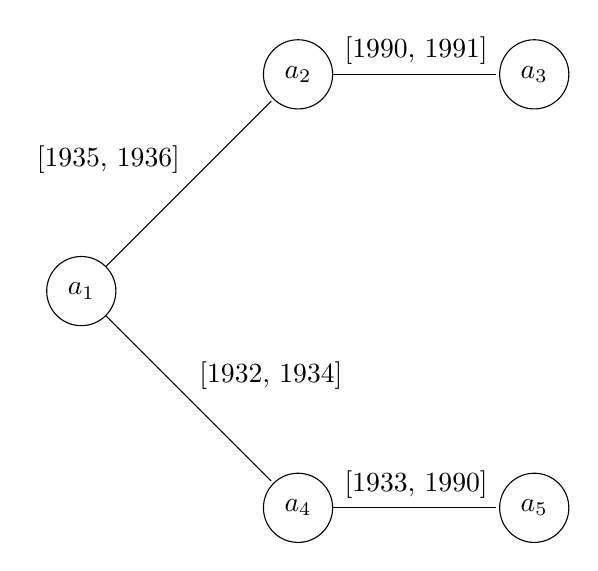
\begin{tikzpicture}[>=stealth',shorten >=1pt,auto,node distance=3cm]
    \node[state]     (a1)                            {$a_1$};
    \node[state]     (a2)     [above right=of a1]    {$a_2$};
    \node[state]     (a3)     [right of=a2]          {$a_3$};
    \node[state]     (a4)     [below right=of a1]    {$a_4$};
    \node[state]     (a5)     [right of=a4]          {$a_5$};

    \path[-]
      (a1) edge             node {[1935, 1936]} (a2)
           edge             node {[1932, 1934]} (a4)
      (a2) edge             node {[1990, 1991]} (a3)
      (a4) edge             node {[1933, 1990]} (a5);
  \end{tikzpicture}
  \caption{Example showing difference in windowed fastest and shortest paths}
  \label{fig:windowed_path_ex}
\end{figure}

In Figure \ref{fig:windowed_path_ex}, there exists a complete contemporary path
$P_1$ such that $P_1 = a_5a_4,a_4a_1$, but there does not exist a complete
contemporary path $P_2$ such that $P_2 = a_5a_4,a_4a_1,a_1a_2$.

\section{ Shortest Path Algorithms}

In this section we present naive shortest path algorithms along with their proofs
based on Dijkstra for consecutive and complete temporal paths. We will analyze
these in the case of the unweighted coauthorship network $(V,E,T)$. They are each
heavily based on the standard Breadth First Search, but performed on edges -
not on vertices.


For both
algorithms we use the matrix \texttt{dist}, which represents a complete mapping
between pairs of vertices and initial time stamp and the distance between them, with the default
value set to $\infty$. Similarly \texttt{interval} is an array representing the
union of all edges on the shortest path to each edge, with the default value
being \texttt{null}. R is a min-heap of edges \texttt{e}, sorted on
\texttt{dist[src][snd e]}.

The last piece of this is the helper-function \texttt{edge\_neighborhood}, which
for an edge $e = (u,v)$ corresponds to the standard mathematical set
$N_e(v) - \{e\}$. This computation will take $O(log m)$ using a B+-Tree index
on the edge set. Its also possible to include an adjacency list in the definition
of an edge, and have \texttt{edge\_neighborhood} pull it out, giving $O(1)$, but
requiring precomputation with cost $O(m\log m)$.
Each algorithm iterates through every vertex, and then in the
worst case, every edge will enter $R$ at some point, giving $O(nm \log m)$. Then
we do this accross all time slices, so we have $O(tnm\log m)$.

\subsection{Consecutive Shortest Path Distance Algorithm}

\begin{algorithm}[H]
\SetAlgoLined
\KwIn{A temporal graph $G = (V, E, T)$ and $dist$ which encapsulates
  a complete mapping between pairs of vertices along with an initial timestamp
  to the distance between them, with the default values set to $\infty$.}
\KwOut{The algorithm outputs $dist$ such that
  $dist[t][v_{src}][v_{dest}] = d$ where $d$ is the (shortest consecutive path)
  distance from node $v_{src}$ to node $v_{dest}$ such that time $t$ intersects the time
  interval of the first edge in the path.}
  \ForEach(//loop over nodes in time slices){
    time, start node pair $(t, v_{src})$ in $\mathcal{T} \times V$
  }{
    Let $e_{src} = (v_{src}, v_{src})$\;
    Let shortest interval be $T(e_{src}) = (t, t)$\;
    Let the reached edges min-heap $R = \{e_{src}\}$\;
    Let the searched edges $S = \varnothing$\;
    Let $dist[t][v_{src}][v_{src}] = 0$\;
    \While{$R \neq \varnothing$}{
      Let $e_{pred} = pop(R)$\;
      Insert $e_{pred}$ into $S$\;
      \ForEach{$e_{succ} = (u,v) \in N_{e_{pred}}(v) - S \cup R$}{
        \If{$T(e_{pred}) \cap T(e_{succ}) \neq \varnothing$}{
          Let $dist[t][v_{src}][v] = min(dist[t][v_{src}][u] + 1, dist[t][v_{src}][v])$\;
          Insert $e_{succ}$ into $R$\;
        }
      }
    }
  }
  \Return{dist}\;
 \caption{Consecutive Shortest Path Distance Algorithm}
\label{fig:consec_STP_alg}
\end{algorithm}

\begin{proof}
  The inductive proof follows by the proof of BFS and the definition of
  consecutive shortest path.
\end{proof}

\subsection{Complete Shortest Path Distance Algorithm}

\section{Fastest Path Algorithms}

\subsection{Consecutive Fastest Path Distance Algorithm}

\subsection{Complete Fastest Path Algorithm}

\end{document}
